\documentclass[11pt]{article}
\usepackage[a4paper, top=2cm, bottom=2cm, left=1.5cm, right=1.5cm]{geometry}

\usepackage{fancyhdr}
\usepackage{lastpage}
\usepackage[showseconds=false,showzone=false]{datetime2}

% First page style - empty
\fancypagestyle{firstpage}{
    \fancyhf{}
    \renewcommand{\headrulewidth}{0pt}
    \renewcommand{\footrulewidth}{0pt}
}
% Running page style with normal header
\fancypagestyle{runningpage}{
    \fancyhf{}
    \fancyhead[L]{\hmwkTitle}
    \fancyhead[R]{\hmwkDueDate}
    \fancyfoot[L]{{\footnotesize Last updated: \DTMnow}}
    \fancyfoot[R]{{\footnotesize Page \thepage\ of \pageref{LastPage}}}
    \renewcommand{\headrulewidth}{0.4pt}
    \renewcommand{\footrulewidth}{0pt}
}

\usepackage{graphicx}
\usepackage{tabularray} % for tables
\usepackage[table]{xcolor}    % loads also colortbl


% Fixed width font
\usepackage{sourcecodepro}

% Java listings
\usepackage{listings}
\lstset{language=[11]C++,
  showspaces=false,
  showtabs=false,
  tabsize=4,
  breaklines=true,
  showstringspaces=false,
  breakatwhitespace=true,
  %commentstyle=\color{green},
  escapeinside={\%*}{*},  % if you want to add LaTeX within your code
  keywordstyle=\ttfamily\bfseries,
  stringstyle=\color{red},
  basicstyle=\ttfamily,%\footnotesize,
  %morekeywords={range,var,in,all,forall,alldifferent,sum,solve}  %,
  %moredelim=[il][\textcolor{pgrey}]{$$},
  %moredelim=[is][\textcolor{pgrey}]{\%\%}{\%\%}
}


\usepackage{amsmath,amssymb}
\usepackage{multicol}

% for algorithms
\usepackage[noend]{algpseudocode}
\algrenewcommand{\algorithmiccomment}[1]{// #1}

\usepackage{url}
\usepackage{hyperref}

% alltt
\usepackage{alltt}


% symbols
%\usepackage{fontawesome}
%\usepackage{textcomp}
%\newcommand\myleaf{\mbox{\footnotesize \textleaf}}



% -------------------------------------------------
%  Miscellaneous commands (from Julian)
% -------------------------------------------------
\newcommand{\str}[1]{\mathsf{#1}}
\newcommand{\set}[1]{\left\{ #1 \right\}}
\newcommand{\sset}[2]{\left\{ #1\, \suchthat\, #2 \right\}}
\newcommand{\suchthat}{|}
\newcommand{\abs}[1]{\left| #1 \right|}
\newcommand{\etal}{\textit{et~al.}}
\newcommand{\ceil}[1]{\left\lceil #1 \right\rceil}
\newcommand{\floor}[1]{\left\lfloor #1 \right\rfloor}
\newcommand{\tuple}[1]{\left( #1 \right)}

\newcommand{\hide}[1]{}

\newcommand{\PP}{\textsf{P}}
\newcommand{\NP}{\textsf{NP}}

%\newcommand{\oT}{{\operatorname{T}}}
\newcommand{\Opt}{{\operatorname{Opt}}}
%\newcommand{\Rs}{{\text{Rs }}}

\newcommand{\sN}{{\operatorname{\mathbb N}}}
\newcommand{\sZ}{{\operatorname{\mathbb Z}}}
\newcommand{\sR}{{\operatorname{\mathbb R}}}
\newcommand{\sQ}{{\operatorname{\mathbb Q}}}

\newcommand{\expected}{{\operatorname{\mathbb E}}}

\newcommand{\cU}{{\mathcal U}}
\newcommand{\cO}{{\mathcal O}}


%%%%%%%%%%%%%%%%%%%%%%%%%%%%%%%
% Homework Details
%%%%%%%%%%%%%%%%%%%%%%%%%%%%%%   

\newcommand{\hmwkTitle}{\emph{Lab\ \#8}}
\newcommand{\hmwkCourseTitle}{Data Structures}
\newcommand{\hmwkCourseCode}{CSE247}
\newcommand{\hmwkSemester}{Fall'25}
%\newcommand{\hmwkMaxMarks}{\emph{Max Marks:} \numpoints}
%\newcommand{\hmwkDueDate}{\emph{Time Allowed:} 10 minutes}
\newcommand{\hmwkMaxMarks}{}
\newcommand{\hmwkDueDate}{Oct 27, 2025}
%\newcommand{\hmwkInstructor}{Dr. Imran Rauf}
%\newcommand{\hmwkTA}{Hamza Fudda}




%%%%%%%%%%%%%%%%%%%%%%%%%%%%%%%%%%%%%%%%%%%%%%%%%%%%%%%%%
%%%%%%%%%%%%%%%%%%%%%%%%%%%%%%%%%%%%%%%%%%%%%%%%%%%%%%%%%
%%%%%%%%%%%%%%%%%%%%%%%%%%%%%%%%%%%%%%%%%%%%%%%%%%%%%%%%%
\begin{document}
\thispagestyle{firstpage}
\pagestyle{runningpage}

% Manual header for first page
\noindent
\begin{tblr}{
    colspec = {X[l,m] X[c,m] X[r,m]},
    rowsep = 0pt,
    colsep = 0pt,
    width = \textwidth
}
    {\includegraphics[height=1.1cm]{../IBA-logo.png} \\ \hmwkTitle}
    &
    {\large \hmwkCourseCode\ \textsc{\hmwkCourseTitle} \\[0.2cm] \hmwkSemester}
    &
    {\includegraphics[height=1cm]{../SMCS-logo.png} \\ \hmwkDueDate}
\end{tblr}

\noindent\rule{\textwidth}{0.4pt}

% Implement a solution to the word puzzle problem described below.
\section*{Word Puzzle Problem}
Consider the problem called \textit{word search}\footnote{\url{https://en.wikipedia.org/wiki/Word_search}}, illustrated in the diagram below.
\begin{center}
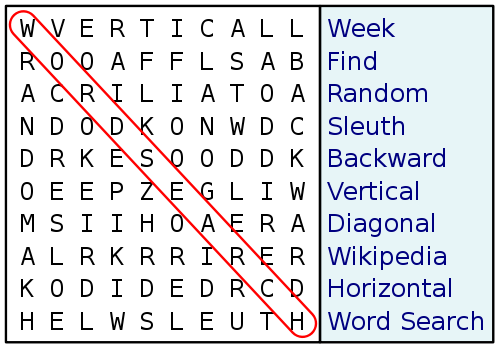
\includegraphics[width=0.4\textwidth]{wordsearch.png}
\end{center}
In this $10 \times 10$ grid of letters, the goal is to find words in the puzzle in any of the eight directions. The word circled in red is in the south-east direction. Words can go backward (although none do in this example), but they cannot ``wrap around'' from one side to the other (or from top to bottom, etc.).

For the purposes of this lab, your program will be presented with a grid of letters and a dictionary of words. All words in the dictionary that are in the grid, in any of the 8 directions, are to be outputted.

A string of letters from the grid will depend on four values:
\begin{itemize}
\item     The $x$ value of the starting letter
\item     The $y$ value of the starting letter
\item     The direction, $d$, of the word (directions can be represented as integers 1-8, if that is easier)
\item     The length, $l$, of the string
\end{itemize}
This implies that your code will have quad-nested \lstinline|for| loops.

A few notes about the length of the words: the program to implement will not consider words of length less than 3, and the maximum word length is a constant (which is defined as the longest word in the input dictionary file provided to the program at run-time).

There are a number of optimizations that one can implement, a few of which are mentioned here. Depending on how you implement them, they may not work all that well, of course.
\begin{itemize}
\item    Choose a good load factor, $\alpha$, for your hash table
\item    Implement a reasonable collision resolution strategy
\item    In addition to storing each word, $W$, you can also store the prefixes of that word. So if the word is ``amazing'', you would store ``ama'', ``amaz'', ``amazi'', ``amazin'', and ``amazing'' in the hash table. There would need to be some way to differentiate between prefixes (``amaz'') and the actual words (``amazing''). This way if you are working in a given direction, and the particular string you are generating is not a prefix, then you know there are no further words in the dictionary in the given direction.
\item    You can keep track of a previous hash to help compute the next one faster. For example, if you have just computed the hash for ``foo'', then you can keep that hash value on hand to compute the hash for ``food'' faster.
\end{itemize}

\section*{Lab task}
For this lab you need to implement a solution to the word puzzle problem described above.

The basic idea is that given a dictionary of words, we want to write a program that finds all instances of those words in a grid of letters. This is similar to the word search puzzles where you circle the words, horizontally, vertically or diagonally in the grid. As specified above, words can appear in any order (including backwards) in the puzzle. However, in our case you are not given the list of words to find, you are merely given the grid and told to find all the English words in the grid. You will be given a dictionary (list) of English words, but you should expect this to be very large. You will want to put this list of words into a hash table to facilitate quickly checking if a particular combination of letters is a word in the dictionary.

You must write your own hash table for this lab. You will be expected to be able to implement a hash table after completing the lab. You should definitely stay away from templates for your implementation. You may use separate chaining with buckets of any type you wish (linked list, etc., but not vectors) or open addressing with any collision resolution strategy you wish (linear probing, quadratic probing, double hashing). The hash table itself will need to be an array or vector (you may use the STL vector for this); your separate chaining secondary data structure may also be from the STL. Thus, you may use any data structures that you want EXCEPT a vector of vectors, which is specifically forbidden. You can use a vector of linked lists, however. Obviously, you cannot use any STL hash table implementation.

Your program MUST take in the file names as command-line parameters, not as inputs to the program. The first is the dictionary file, the second is the grid file. Indeed, the program will ask for NO input, as the two inputs necessary (the two file names) are passed in as command-line parameters. See the \texttt{cmdlineparams.cpp} file for an example of how to do this.

The task for the lab is to get the code working. Optimization (reducing memory use, choosing the right collision resolution method, the right secondary data structure, different hash functions, etc.) is left as optional homework. 

As discussed in lecture, a hash table needs to be a prime number in size in order to work. You can adapt the code in the \texttt{primenumber.cpp} file to determine the next highest prime number (of course, the next highest prime number is determined after you double the size of your original hash table).

We provide you with a second \texttt{C++} file, \texttt{getWordInGrid.cpp}, that provides two useful functions. The first is \texttt{readInGrid()}, which will read in a grid file using \texttt{C++} streams. The grid file format (specified below) is very specific, and this code follows that specification. The second function, \texttt{getWordInGrid()}, will return a word in a 2-D grid of letters in a given direction. Extensive comments in the \texttt{getWordInGrid.cpp} file explain how to use these functions. 

Somehow your program will need to handle input dictionaries of various sizes, and creating the appropriate size hash table. To get the program working the first time, you can just hard code a prime number table size. But at some point, you will have to handle different size hash tables.
\begin{itemize}
\item    One option is to implement a \lstinline|rehash()| function that will double the size of the array, hash all the old values into the new table, and then remove the old table.
\item    A second option is to do two passes through the dictionary file. The first time you count the number of elements, use that to create an appropriate sized hash table, and the second time through the dictionary file you insert all the words into the table itself.
\end{itemize}

Note that you do not have to implement \lstinline|remove()| functionality for your hash table.

\subsection*{Submission requirements}

You should submit the following files:
\begin{itemize}
    \item \texttt{wordPuzzle.cpp}: contains the \lstinline|main()| method
    \item \texttt{stopWatch.hpp}: the code you downloaded for this lab; this file does not need any modifications
    \item \texttt{hashTable.hpp/cpp}: the code for your hash table
\end{itemize}

You can submit other files, if you want. Your program should conform to the input and output requirements listed in the lab procedure, discussed below, as that is how it will be tested. 

\subsection*{Program Details}
\begin{itemize}
\item \textbf{Input grids:} You can expect an input text file in which the first line is the number of rows, and the second is the number of columns. The third line is the grid data, with no spaces (i.e. it will be rows X cols number of characters). Several example grids available. 
%Grids will not include whitespace, numbers, punctuation, or special characters.

\item \textbf{Dictionary files:} The dictionary can be assumed to contain one word per line. The longest word in our data files is 22 letters. Words which contain a space or other special character (\& or ' or -) or number may occur in the dictionary, but would never appear in a valid grid. Your program should be able to handle dictionaries with such words, although you are not required to put them into the hash table.

\item \textbf{Timing:} Timer routines are available in the provided source code (timer.cpp (src), timer.h (src), and timer\_test.cpp (src)). We are interested in timing how long it takes to find all valid words in a grid. We are NOT interested in how long it takes to fill up the hash table initially. Therefore you need to place your timing calls around the outermost loop that contains code in which the grid is actually searched.

\item \textbf{Valid words:} Your program should only report words with three or more letters -- there are simply too many hits if one and two letter words are allowed, and it's difficult to judge correctness, even on very small word searches. This size (i.e. 3) can be hard-coded into your program. Depending on how you've implemented your loop, this could be something as simple as a single test and a continue statement. One and two letter words may occur in the dictionary file, but you are not required to put them in your hash table (although it is fine to do so).

\item \textbf{Upper case / lower case:} You should be prepared for any English language alphabet characters of both cases. Searches are case-sensitive. Thus, if the word in the dictionary is 'Foo', it should not register a match to the text 'foo' in the grid.

\item \textbf{Duplicates:} If a word occurs more than once in a grid, then each instance should be treated as a separate word.
\end{itemize}

\subsection*{Output format}
In an effort to make it easier to determine if the program is working properly or not, we want to standardize the output format. Below is the \texttt{4x7.out.txt} file:
\begin{alltt}
N (3, 2):       text
E (0, 3):       sod
N (2, 5):       fad
E (1, 0):       pax
NW(3, 6):       eft
E (2, 0):       ace
W (2, 4):       tee
NE(2, 4):       tat
SW(0, 6):       tat
9 words found
Found all words in 0.000835 seconds
\end{alltt}

We aren't so worried about the exact spacing, as we can easily (and automatically) ignore that when comparing your output to the desired output. But the characters and punctuation should all be the same. Note that the order the words are found does not matter, although they should all be listed before the last 2 summary lines at the bottom. You can directly compare your output to the expected output (while ignoring spaces and word order).

\subsection*{Execution}
We are going to compile your code as follows:
\begin{alltt}
g++ -O2 -o lab08.exe wordPuzzle.cpp hashTable.cpp
\end{alltt}
It can then be executed as follows:
\begin{alltt}
lab08.exe <dictionary_file> <grid_file>
\end{alltt}

\quad If your program attempts to get the dictionary file and grid file through standard input, it will not work properly and you will lose all credit. So be sure to use command-line parameters! See the section on handling command-line parameters, above.





\end{document}